\documentclass[12pt, a4paper, oneside]{ctexart}
\usepackage{amsmath, amsthm, amssymb, graphicx}
\usepackage[bookmarks=true, colorlinks, citecolor=blue, linkcolor=black]{hyperref}
\usepackage[margin = 25mm]{geometry}
\usepackage{setspace}
\usepackage{listings}
\usepackage{ctex}
\usepackage{float}
\usepackage{xcolor}

\definecolor{codegreen}{rgb}{0,0.6,0}
\definecolor{codegray}{rgb}{0.5,0.5,0.5}
\definecolor{codepurple}{rgb}{0.58,0,0.82}
\definecolor{backcolour}{rgb}{0.95,0.95,0.92}

\lstdefinestyle{mystyle}{
    backgroundcolor=\color{backcolour},   
    commentstyle=\color{codegreen},
    keywordstyle=\color{magenta},
    numberstyle=\tiny\color{codegray},
    stringstyle=\color{codepurple},
    basicstyle=\ttfamily\footnotesize,
    breakatwhitespace=false,         
    breaklines=true,                 
    captionpos=b,                    
    keepspaces=true,                 
    numbers=left,                    
    numbersep=5pt,                  
    showspaces=false,                
    showstringspaces=false,
    showtabs=false,                  
    tabsize=2
}

\lstset{style=mystyle}


\title{ADI方法数值求解二维平面传热问题}
\date{\today}
\author{202011010101物理2001孙陶庵}
\begin{document}
\begin{spacing}{2.0}
\tableofcontents
\maketitle

\section{问题}
求以下PDE的数值解:
$\displaystyle \frac{\partial T}{\partial t} = \kappa (\frac{\partial^2 T}{\partial x^2} + \frac{\partial^2 T}{\partial y^2})$
其中初始条件区域内的温度为$0^{\circ}C$
板子长宽皆为$25cm$
边界条件上下左右四边分别有恒定温度:$100^{\circ}C, 0^{\circ}C, 75^{\circ}C, 50^{\circ}C$
matlab用ADI方法求温度分布随时间的变化画出3D图形


\section{ADI方法}
1.将二维平面分割成多个小方格。在每个小方格中,u、x和y分别离散化为U(i,j)、X(i,j)和Y(i,j),其中i和j分别表示x和y的离散坐标。

2.使用ADI方法对每个小方格进行求解。
即将二维热传导方程分解为两个一维问题。在每个方向上,可以使用隐式方法进行时间步进,并使用三对角矩阵算法来解决空间离散化问题。每次迭代后,将得到一个新的温度场U(i,j)。
根据所得到的温度场,计算需要的热量分布、温度梯度等。
这里求解三对角矩阵是用的高斯消元法,简单来说就构造增广矩阵进行行变换后将线性方程组转化为一个上三角矩阵,进而通过回带求解得到方程组的解。
以下是推导过程:\\
考虑二维热传导方程:

\begin{center}
    $\displaystyle \frac{\partial u}{\partial t} = k\left(\frac{\partial^2 u}{\partial x^2} + \frac{\partial^2 u}{\partial y^2}\right)$
\end{center}

其中,$u$ 是温度,$t$ 是时间,$k$ 是热传导系数,$x$ 和 $y$ 是空间坐标。

ADI 方法求解方程,需要将其分解为两个一维问题,一个在 $x$ 方向,一个在 $y$ 方向。具体地,我们可以将时间步长 $\Delta t$ 分成两个部分,
即 $\Delta t/2$,然后在 $x$ 方向应用隐式 Euler 方法,得到一个中间温度场 $u^{n+1/2}_{i,j}$,然后在 $y$ 方向应用隐式 Euler 方法,
得到下一个时间步长的温度场 $u^{n+1}_{i,j}$。

1.在 $x$ 方向上,将 $u^{n}_{i,j}$ 的值用 $u^{n+1/2}_{i,j}$ 表示,即
\begin{center}
    $\displaystyle u^{n}_{i,j} \approx u^{n+1/2}_{i,j}$
\end{center}

2.将 (2) 代入二维热传导方程中,得到
\begin{center}
    $\displaystyle \frac{\partial u^{n+1/2}_{i,j}}{\partial t} = k\left(\frac{\partial^2 u^{n+1/2}_{i,j}}{\partial x^2} + \frac{\partial^2 u^{n}_{i,j}}{\partial y^2}\right)$
\end{center}

3.在 $x$ 方向上,应用隐式 Euler 方法,得到
\begin{center}
    $\displaystyle u^{n+1/2}_{i,j} - u^{n}_{i,j} = \frac{\Delta t}{2} k\frac{\partial^2 u^{n+1/2}_{i,j}}{\partial x^2}$
\end{center}

4.在 $y$ 方向上,将 $u^{n+1/2}_{i,j}$ 的值用 $u^{n+1/2}_{i,j+1}$ 表示,即
\begin{center}
    $\displaystyle u^{n+1/2}_{i,j} \approx u^{n+1/2}_{i,j+1}$
\end{center}

5.将 (4) 代入 (2) 中,得到
\begin{center}
    $\displaystyle \frac{\partial u^{n+1/2}_{i,j+1}}{\partial t} = k\left(\frac{\partial^2 u^{n+1/2}_{i,j}}{\partial x^2} + \frac{\partial^2 u^{n+1/2}_{i,j+1}}{\partial y^2}\right)$
\end{center}
6.在 $y$ 方向上,应用隐式 Euler 方法,得到
\begin{center}
    $\displaystyle u^{n+1}_{i,j} - u^{n+1/2}_{i,j+1} = \frac{\Delta t}{2} k\frac{\partial^2 u^{n+1/2}_{i,j+1}}{\partial y^2}$
\end{center}

7.将 (3) 和 (6) 相加,得到
\begin{center}
    $\displaystyle u^{n+1}_{i,j} - u^{n}_{i,j} = \frac{\Delta t}{2} k\left(\frac{\partial^2 u^{n+1/2}_{i,j}}{\partial x^2} + \frac{\partial^2 u^{n+1/2}_{i,j+1}}{\partial y^2}\right)$
\end{center}

8.将 $u^{n+1/2}_{i,j}$ 和 $u^{n+1/2}_{i,j+1}$ 的值用 $u^{n+1}_{i,j+1/2}$ 表示,即
\begin{center}
    $\displaystyle u^{n+1/2}_{i,j} \approx u^{n+1}_{i,j+1/2}$
\end{center}

\begin{center}
    $\displaystyle u^{n+1/2}_{i,j+1} \approx u^{n+1}_{i,j+1/2}$
\end{center}

9.将 (8) 代入 (7) 中,得到
\begin{center}
    $\displaystyle u^{n+1}_{i,j} - u^{n}_{i,j} = \frac{\Delta t}{2} k\left(\frac{\partial^2 u^{n+1}_{i,j+1/2}}{\partial x^2} + \frac{\partial^2 u^{n+1}_{i,j+1/2}}{\partial y^2}\right)$
\end{center}

10.最终得到 ADI 方法的迭代公式:
\begin{center}
    $\displaystyle u^{n+1}_{i,j} = u^{n}_{i,j} + \frac{\Delta t}{2} k\left(\frac{u^{n+1}_{i+1,j} - 2u^{n+1}_{i,j} + u^{n+1}_{i-1,j}}{\Delta x^2} + \frac{u^{n+1}_{i,j+1} - 2u^{n+1}_{i,j} + u^{n+1}_{i,j-1}}{\Delta y^2}\right)$
\end{center}

其中,$u^{n+1}_{i,j}$ 表示下一个时间步长的温度场,$u^{n}_{i,j}$ 表示当前时间步长的温度场,$\Delta x$ 和 $\Delta y$ 分别是 $x$ 和 $y$ 方向的网格间距。该公式是一个中心差分格式,可以用于数值计算二维平面传热问题。



1.在x方向走半个时间步
\begin{center}
    $\displaystyle \frac{u_{i,j}^{k+1/2}-u_{i,j}^{k}}{\Delta t/2}=\kappa\left(\frac{u_{i+1,j}^{k+1/2}-2u_{i,j}^{k+1/2}+u_{i-1,j}^{k+1/2}}{\left(\Delta x\right)^{2}}+\frac{u_{i,j+1}^{k}-2u_{i,j}^{k}+u_{i,j-1}^{k}}{\left(\Delta y\right)^{2}}\right)$
\end{center}
2.在y方向走半个时间步
\begin{center}
    $\displaystyle \frac{u_{i,j}^{k+1}-u_{i,j}^{k+1/2}}{\Delta t/2}=\kappa\left(\frac{u_{i+1,j}^{k+1/2}-2u_{i,j}^{k+1/2}+u_{i-1,j}^{k+1/2}}{\left(\Delta x\right)^{2}}+\frac{u_{i,j+1}^{k+1}-2u_{i,j}^{k+1}+u_{i,j}^{k+1}}{\left(\Delta y\right)^{2}}\right)$
\end{center}
取$\displaystyle \Delta x=\Delta y,r=\frac{\kappa\Delta t}{\left(\Delta x\right)^{2}}$则方程变为:\\
$\displaystyle -ru_{i-1}^{k+1/2}+2(1+r)u_{i,j}^{k+1/2}-ru_{i+1}^{k+1/2}=ru_{i,j-1}^{k}+2(1-r)u_{i,j}^{k}+ru_{j+1}^{k}\\ -ru_{i,j-1}^{k+1}+2(1+r)u_{i,j}^{k+1}-ru_{i,j+1}^{k+1}=ru_{i-1}^{k+1/2}+2(1-r)u_{i,j}^{k+1/2}+ru_{i+1}^{k+1/2}$



\section{代码部分}

\begin{lstlisting}
L = 25;
W = 25; 
T = 1;
Nx = 21;
Ny = 21; 
Nt = 1000;
dx = L / (Nx - 1);
dy = W / (Ny - 1); 
dt = T / Nt; 
kappa = 0.835;
u0 = zeros(Nx, Ny);
u0(ceil(Nx/2), ceil(Ny/2)) = 0;
u0(:, 1) = 75; 
u0(:, end) = 50;
u0(1, :) = 100;
u0(end, :) = 0; 

%zhushi
ax = dt * kappa / (2 * dx^2);
ay = dt * kappa / (2 * dy^2);
bx = 1 + 2 * ax;
by = 1 + 2 * ay;
cx = 1 - 2 * ax;
cy = 1 - 2 * ay;

for k = 1:Nt
    % alphazhushi
    for i = 2:Nx-1
        a = zeros(Ny-2, Ny-2);
        b = zeros(Ny-2, 1);
        % zhushialpha
        for j = 2:Ny-1
            a(j-1, j-1) = bx;
            if j > 2
                a(j-1, j-2) = cx * ax;
            end
            if j < Ny-1
                a(j-1, j) = cx * ax;
            end
            b(j-1) = cy * u0(i-1, j) + (1 - 2*cy) * u0(i, j) + cy * u0(i+1, j);
        end
        % aaa1122
        u1(i, 2:Ny-1) = GaussElimination(a, b);
    end
    % ylpha
    for j = 2:Ny-1
        a = zeros(Nx-2, Nx-2);
        b = zeros(Nx-3, 1);
        % zhushialpha
        for i = 2:Nx-1
            a(i-1, i-1) = by;
            if i > 2
                a(i-1, i-2) = cy * ay;
            end
            if i < Nx-1
                a(i-1, i) = cy * ay;
            end
            b(i-1) = cx * u1(i, j-1) + (1 - 2*cx) * u1(i, j) + cx * u1(i, j+1);
        end
        % aaa1122
        u0(2:Nx-1, j) = Thomas(a, b);
    end
end

[X, Y] = meshgrid(0:dx:L, 0:dy:W);
surf(X, Y, u0');
xlabel('x');
ylabel('y');
zlabel('Temperature');



function x = GaussElimination(A, b)

n = size(A, 1);
m = size(b, 2);

if n ~= m
    error('Error: The size of A and b do not match.');
end

% aa55688
for i = 2:n
    factor = A(i, i-1) / A(i-1, i-1);
    A(i, i-1) = 0;
    A(i, i) = A(i, i) - factor * A(i-1, i);
    b(i) = b(i) - factor * b(i-1);
end

% pa89
x(n) = b(n) / A(n, n);
for i = n-1:-1:1
    x(i) = (b(i) - A(i, i+1) * x(i+1)) / A(i, i);
end

x = x';
end
\end{lstlisting}
注释部分:\\
zhushi:定义AD方程的系数矩阵;
alphazhushi:按x方向迭代;
zhushialpha:构建三对角矩阵;
aaa1122:解三对角矩阵方程;
ylpha:按y方向迭代;
aa55688:前向消元;
pa89:回代求解;



最后形成这张图片
\begin{figure}[htbp][H]
    \centering
    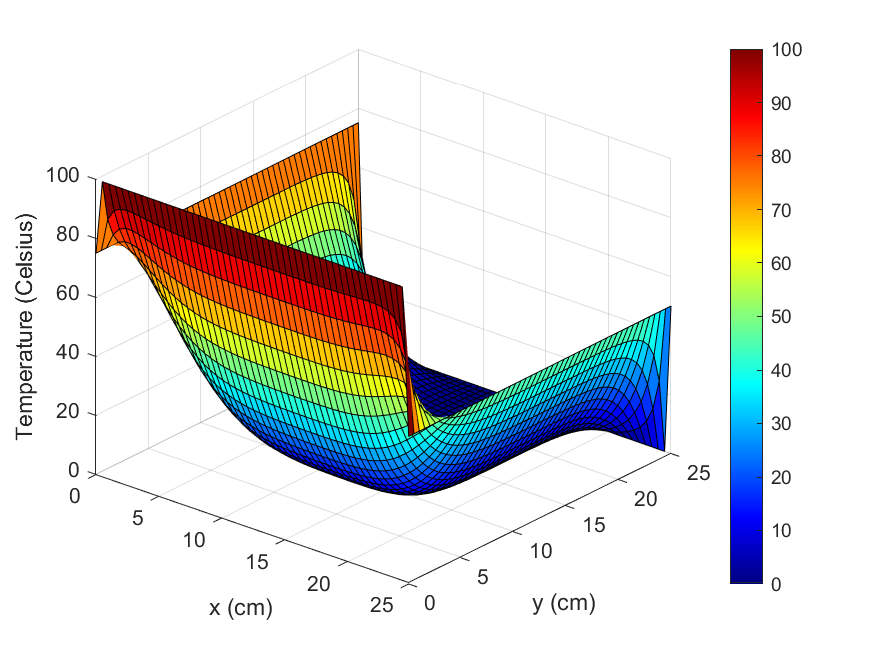
\includegraphics[width=8cm]{frame_1.png}
    \caption{结果}
\end{figure}

\section{t=1s时的温度分布}
备注:这是最一开始的代码,原本以为只要求$t=1s$时的温度分布,后面才发现要全部的,所以又重新写了一份在上面
\begin{lstlisting}
L = 0.25; 
dx = 0.01; dy = 0.01;  
dt = 0.01; 
kappa = 0.835; 
T_ini = zeros(L/dx, L/dy); 

T_ini(1, :) = 100;  % up
T_ini(end, :) = 0;  % down
T_ini(:, 1) = 75;  % left
T_ini(:, end) = 50;  % right


t_start = 0;
t_end = 1;
t_range = t_start:dt:t_end;

T = T_ini;
for t = t_range
    % zhushialpha
    a = kappa * dt / dx^2;
    %ax = ay = r
    r = a;
    [m, n] = size(T);
    A = zeros(m*n, m*n);
    b = zeros(m*n, 1);
    for i = 1:m
        for j = 1:n
            idalpha = (i-1)*n + j;
            if i == 1 || i == m || j == 1 || j == n
                A(idalpha, idalpha) = 1;
                b(idalpha) = T(i, j);
            else
                A(idalpha, idalpha-n) = -r;
                A(idalpha, idalpha-1) = -1;
                A(idalpha, idalpha) = 2*(1+r);
                A(idalpha, idalpha+1) = -1;
                A(idalpha, idalpha+n) = -1/r;
                b(idalpha) = T(i-1, j)*r + T(i, j-1) + T(i, j+1) + T(i+1, j)/r;
            end
        end
    end
    
    %Temp. Distribution
    T_new = reshape(A\b, m, n);
    T = T_new;
end


imagesc([0 L], [0 L], T);
set(gca, 'YDir', 'reverse')
colormap(jet);
colorbar;
title('Temperature Distribution at t=1');
xlabel('x (m)');
ylabel('y (m)');


\end{lstlisting}
最后形成这张图片
\begin{figure}[htbp][H]
    \centering
    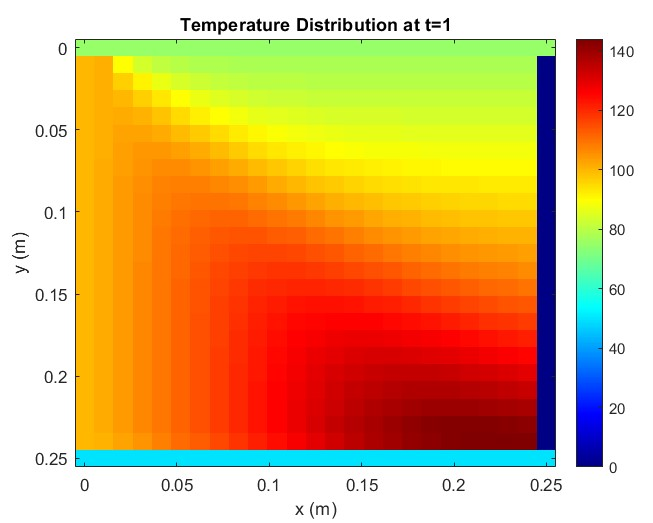
\includegraphics[width=8cm]{t=1.jpg}
    \caption{结果}
\end{figure}
\section{特别}
在代码后面加上特定内容可以把要求的图做成多张图片,再透过python代码整合成GIF(附件),可以得到温度随时间的变化。
但是我这里代码无法继续加了(不会做),所以用FTCS方法实现
\begin{lstlisting}
    import numpy as np
import matplotlib.pyplot as plt
from mpl_toolkits.mplot3d import Axes3D
import imageio
import os

L = 25 
n = 50 
dx = L / (n - 1) 
kappa = 0.835  
sigma = 0.25  
dt = sigma * dx**2 / kappa 
T = np.zeros((n, n))
T[0, :] = 100
T[-1, :] = 0 
T[:, 0] = 75
T[:, -1] = 50


total_frames = 15


frames = []
frame_count = 0
for j in range(int(6000)):
    for i in range(1, n-1):
        for k in range(1, n-1):
            T[i, k] += sigma * kappa * (T[i+1, k] - 2*T[i, k] + T[i-1, k] + T[i, k+1] - 2*T[i, k] + T[i, k-1])

    if j % 50 == 0 and frame_count < total_frames:
        frame_count += 1
        x = np.linspace(0, L, n)
        y = np.linspace(0, L, n)
        X, Y = np.meshgrid(x, y)

        fig = plt.figure()
        ax = plt.axes(projection='3d')
        ax.plot_surface(X, Y, T, cmap='viridis')
        ax.set_xlabel('x (cm)')
        ax.set_ylabel('y (cm)')
        ax.set_zlabel('Temperature (Celsius)')

        fig.canvas.draw()
        img = np.frombuffer(fig.canvas.tostring_rgb(), dtype=np.uint8)
        img = img.reshape(fig.canvas.get_width_height()[::-1] + (3,))
        frames.append(img)

        plt.close()

        if frame_count >= total_frames:
            break

imageio.mimsave('temperature.gif', frames, fps=3)
file_path = os.path.join("C:/Users/toby1/Desktop", "temperature.gif")
imageio.mimsave(file_path,frames, fps=10)





\end{lstlisting}



\end{spacing}{}

\end{document}